\subsection{Chaining} 

In addition to the number of arguments, another source of complexity in aliases (i.e. value length) is command composition or chaining.
\num{351060} aliases (\per{7.36}) are composed of more than one command.
The most popular way to combine commands is with a pipe (\verb!|!), used by \per{35.2} of multi-command aliases, closely followed by logical conjunction (\verb|&&|), used by \per{29.75}, and simple chaining (\verb|;|), used by \per{28.4}.
Other operators (\verb|&|, \verb!||!, \verb!|&!) appear in only \per{6.65} of multi-command aliases.
\Cref{tab:operators} shows the top commands in 2nd, 3rd and 4th position of a command chain, for each possible preceding operator.

\begin{table}[h]
	\caption{Top commands following operators}
	\label{tab:operators}
	\begin{tabular}{ll|l|l}    
		\toprule
		& 2nd position & 3rd position & 4th position \\
		\midrule
		\verb!|! & \verb|grep| {\small (\num{34.17})} & \verb|grep| {\small (\num{14.56})} & \verb|xargs| {\small (\num{19.25})} \\     
		& \verb|sort| {\small (\num{11.1})} & \verb|head| {\small (\num{12.37})}& \verb|head| {\small (\num{17.52})}\\ 
		& \verb|xargs| {\small (\num{6.4})} & \verb|sort| {\small (\num{8.81})} & \verb|grep| {\small (\num{11.35})}\\ 
		\midrule
		\verb!&&! & \verb|git| {\small (\num{16.73})} & \verb|git| {\small (\num{16.26})} & \verb|git| {\small (\num{12.47})} \\ 
		& \verb|killall| {\small (\num{8.81})} & \verb|aur| {\small (\num{16.05})} & \verb|date| {\small (\num{8.25})}\\ 
		& \verb|abs| {\small (\num{8.57})} & \verb|startpost| {\small (\num{4.51})} & \verb|brew| {\small (\num{6.44})} \\ 
		\midrule
		\verb!;! & \verb|git| {\small (\num{8.53})} & \verb|zeus| {\small (\num{10.18})} & \verb|brew| {\small (\num{9.29})}\\ 
		& \verb|echo| {\small (\num{6.63})}& \verb|git| {\small (\num{10.06})}  & \verb|echo| {\small (\num{8.15})} \\ 
		&  \verb|cd| {\small (\num{4.84})} & \verb|cd| {\small (\num{5.74})} &  \verb|git| {\small (\num{6.49})}\\ 
		\midrule
		\verb!||! & \verb|alias| {\small (\num{46.37})} & \verb|echo| {\small (\num{18.86})} & \verb|echo| {\small (\num{20.67})} \\ 
		& \verb|tmux| {\small (\num{19.26})} & \verb|tmux| {\small (\num{8.32})}  &  \verb|cd| {\small (\num{20.11})} \\ 
		& \verb|true| {\small (\num{4.56})} &  \verb|umount| {\small (\num{7.41})} & \verb|true| {\small (\num{13.41})}\\ 
		\midrule
		\verb!&! & \verb|disown| {\small (\num{15.12})} & \verb|disown| {\small (\num{16.92})} & \verb|amp| {\small (\num{7.51})} \\
		& \verb|/dev/null| {\small (\num{13.65})} & \verb|!| {\small (\num{6.95})} & \verb|disown| {\small (\num{7.51})} \\
		& \verb|~/X| {\small (\num{5.49})} & \verb|exit| {\small (\num{4.51})} & \verb|exit| {\small (\num{6.36})} \\    
		\midrule
		\verb!|&! & \verb|less| {\small (\num{71.53})} & \verb|grep| {\small (\num{61.54})} & \verb|tee| {\small (\num{100.0})} \\
		& \verb|tee| {\small (\num{11.81})}  & \verb|less| {\small (\num{15.38})} &  \\
		& \verb|grep| {\small (\num{9.03})} & \verb|color| {\small (\num{7.69})} &  \\
		\midrule
	\end{tabular}
\end{table}

% I think this table might be misleading, because it ranks commands by relative occurrence with operators, rather then normalizing with overall command occurrence. That's probably why git dominates &&


The most interesting operator is certainly the pipe (\verb!|!), since it creates an interface between two otherwise separate programs.
\Cref{fig:flow} shows a flow diagram of the top 200 pipelines with three commands that make up at least \per{10} of one participating command's usage.

\begin{figure*}[h]
	\centering    
	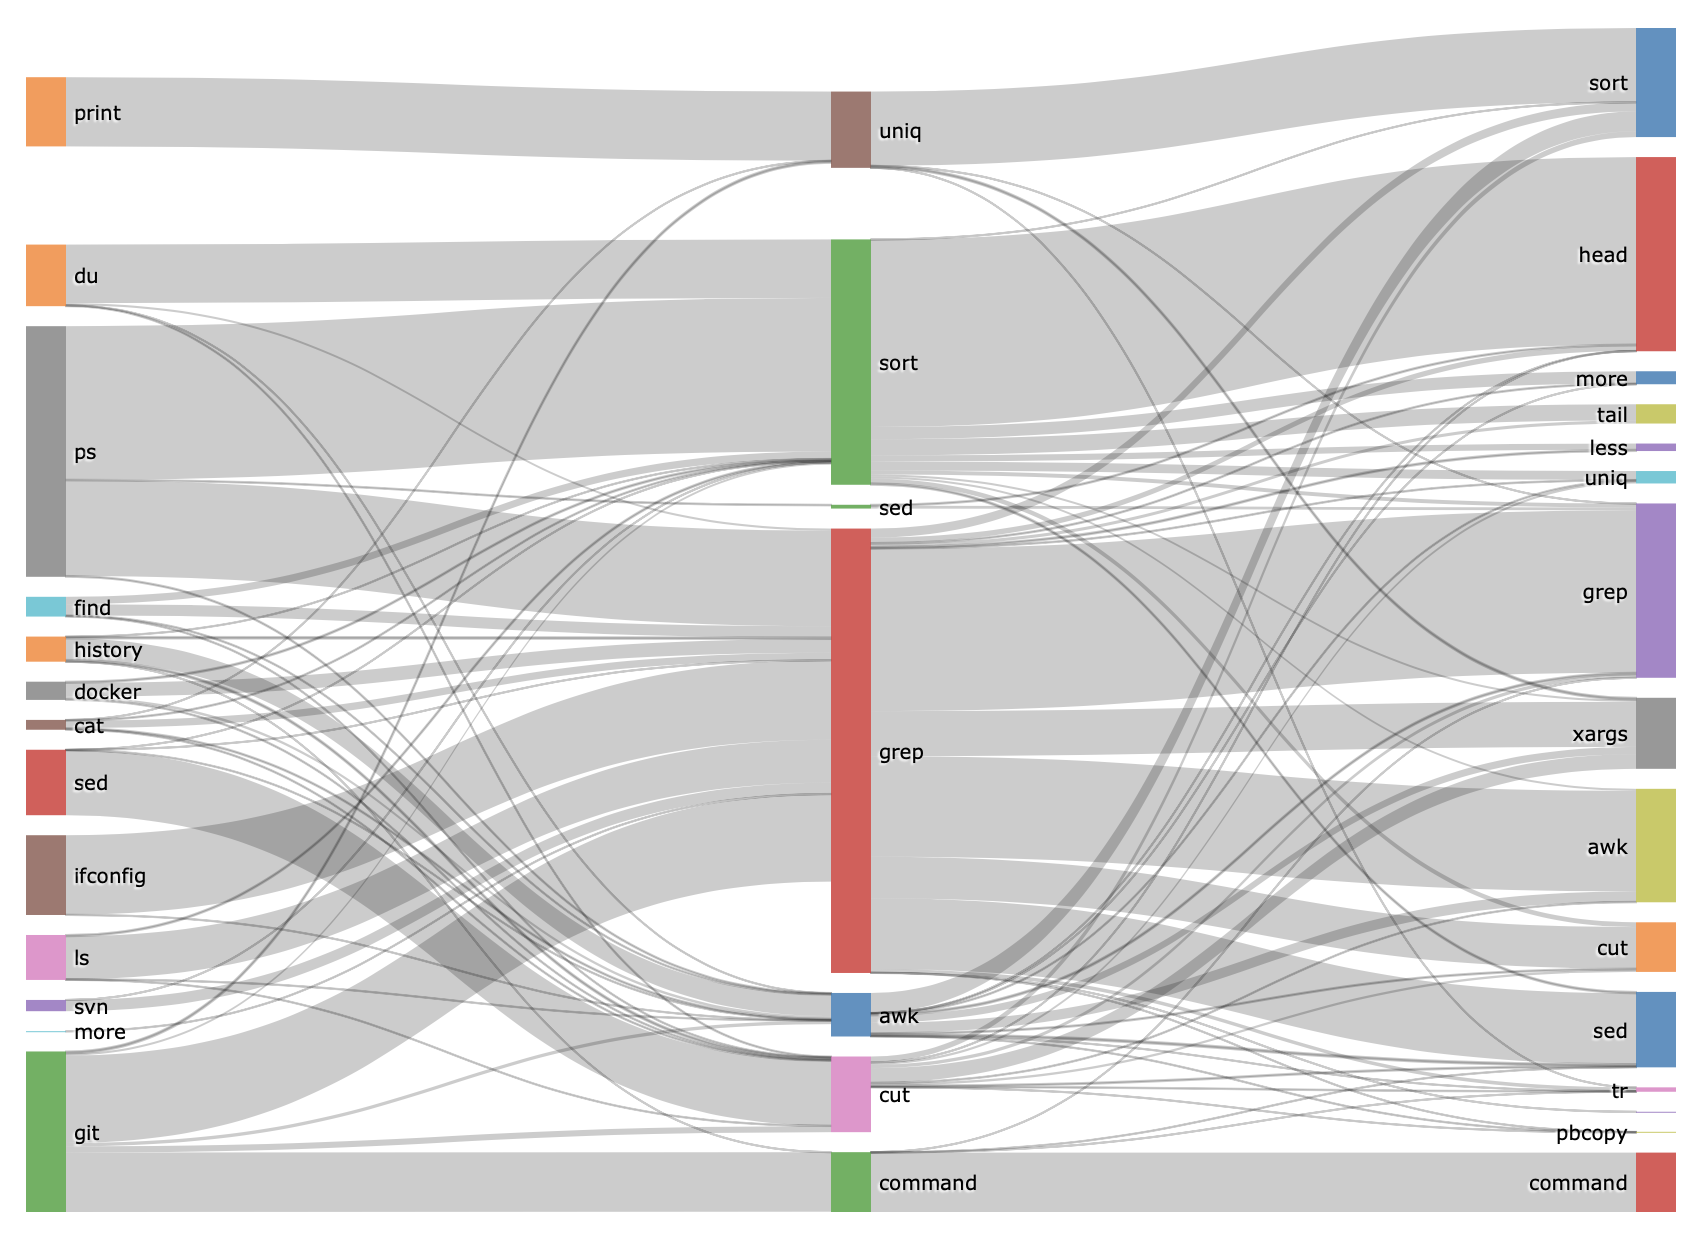
\includegraphics[width=0.8\linewidth]{flow.png}
	\caption{Flow diagram for top 3-command pipelines}
	\label{fig:flow}
\end{figure*}
